% =========================================================================
%  Memory Management in Macaulay2:
%  The Garbage Collector Today, and a Plan to Confine It
%
%  Prepared for the Macaulay2 engine group.
%  Drafted by Andrew Tawfeek with Claude (Fable 5), from the July 2026
%  engine-meeting transcript and direct inspection of the source tree.
%
%  Build:  pdflatex (twice)  or  latexmk -pdf M2-gc-state-and-plan.tex
% =========================================================================
\documentclass[11pt,oneside]{report}

% ---------- fonts & layout ----------
\usepackage[T1]{fontenc}
\usepackage[utf8]{inputenc}
\usepackage{lmodern}
\usepackage{amsmath,amssymb}
\usepackage{microtype}
\usepackage[margin=1in]{geometry}
\usepackage{parskip}
\emergencystretch=1.5em

% ---------- color palette ----------
\usepackage[table]{xcolor}
\definecolor{m2blue}{RGB}{28,80,138}    % headings, links
\definecolor{m2slate}{RGB}{68,84,106}   % secondary text
\definecolor{gcgold}{RGB}{176,137,30}   % GC-heap shading in figures
\definecolor{boxblue}{RGB}{239,244,250}
\definecolor{boxblueframe}{RGB}{163,190,219}
\definecolor{boxamber}{RGB}{252,246,231}
\definecolor{boxamberframe}{RGB}{219,190,120}
\definecolor{boxred}{RGB}{251,238,238}
\definecolor{boxredframe}{RGB}{204,132,132}
\definecolor{boxgreen}{RGB}{238,246,238}
\definecolor{boxgreenframe}{RGB}{140,180,140}
\definecolor{codegray}{RGB}{95,99,104}
\definecolor{codebg}{RGB}{247,247,245}

% ---------- tables, lists, figures ----------
\usepackage{booktabs}
\usepackage{array}
\usepackage{enumitem}
\setlist{topsep=2pt,itemsep=2pt,parsep=0pt}
\usepackage{graphicx}
\usepackage[font=small,labelfont=bf]{caption}
\usepackage{tikz}
\usetikzlibrary{arrows.meta,positioning,fit,backgrounds,calc}

% ---------- boxes ----------
\usepackage[most]{tcolorbox}
\newtcolorbox{inbrief}{colback=boxblue,colframe=boxblueframe,
  title=\textbf{In brief},coltitle=black,colbacktitle=boxblueframe!55!white,
  fonttitle=\sffamily\small,boxrule=0.6pt,arc=2pt,left=6pt,right=6pt,
  top=4pt,bottom=4pt,breakable}
\newtcolorbox{plainterms}{colback=boxgreen,colframe=boxgreenframe,
  title=\textbf{In plain terms},coltitle=black,colbacktitle=boxgreenframe!55!white,
  fonttitle=\sffamily\small,boxrule=0.6pt,arc=2pt,left=6pt,right=6pt,
  top=4pt,bottom=4pt,breakable}
\newtcolorbox{warstory}{colback=boxred,colframe=boxredframe,
  title=\textbf{A cautionary tale},coltitle=black,colbacktitle=boxredframe!55!white,
  fonttitle=\sffamily\small,boxrule=0.6pt,arc=2pt,left=6pt,right=6pt,
  top=4pt,bottom=4pt,breakable}
\newtcolorbox{mikesays}[1][]{colback=boxamber,colframe=boxamberframe,
  title={\textbf{What Mike asked for}\hfill{\normalfont\footnotesize #1}},
  coltitle=black,colbacktitle=boxamberframe!45!white,
  fonttitle=\sffamily\small,boxrule=0.6pt,arc=2pt,left=6pt,right=6pt,
  top=4pt,bottom=4pt,breakable}

% ---------- code ----------
\usepackage{listings}
\lstset{
  language=C++,
  basicstyle=\ttfamily\small,
  keywordstyle=\color{m2blue},
  commentstyle=\color{codegray}\itshape,
  stringstyle=\color{m2slate},
  backgroundcolor=\color{codebg},
  frame=single, rulecolor=\color{black!25},
  framesep=4pt, xleftmargin=6pt, xrightmargin=6pt,
  breaklines=true, showstringspaces=false,
  columns=fullflexible, keepspaces=true,
  aboveskip=8pt, belowskip=8pt
}

% ---------- colored structure ----------
\definecolor{m2code}{RGB}{23,88,124}    % inline identifiers
\definecolor{m2file}{RGB}{72,110,62}    % file paths
\usepackage{sectsty}
\chapterfont{\color{m2blue}}
\sectionfont{\color{m2blue}}
\subsectionfont{\color{m2blue}}

% inline identifiers and file paths
\newcommand{\code}[1]{\textcolor{m2code}{\texttt{#1}}}
\newcommand{\file}[1]{\textcolor{m2file}{\texttt{#1}}}
% striped tables
\usepackage{multicol}

% ---------- hyperref (last) ----------
\usepackage[colorlinks=true,linkcolor=m2blue,urlcolor=m2blue,citecolor=m2blue]{hyperref}

% =========================================================================
\begin{document}

% ---------------- title ----------------
\begin{titlepage}
\centering
\vspace*{2.2cm}
{\LARGE\bfseries Memory Management in Macaulay2\par}
\vspace{0.5cm}
{\Large The Garbage Collector Today,\\[2pt] and a Plan to Confine It\par}
\vspace{1.6cm}
{\large Prepared for the Macaulay2 engine group\par}
\vspace{0.4cm}
{\normalsize Andrew Tawfeek, with Claude (Fable~5)\par}
\vspace{0.4cm}
{\normalsize July 21, 2026 \,\textperiodcentered\, draft for discussion\par}
\vfill
\begin{minipage}{0.86\textwidth}
\small\itshape
Chapter 1 describes, in plain language but with full technical detail, how
memory is actually managed in Macaulay2 today. Chapter 2 is an architectural
plan for confining the garbage collector to the front end, addressing the
requests Mike Stillman made at the July 2026 engine meeting.
\end{minipage}
\vspace{1.2cm}
\end{titlepage}

% ---------------- preface ----------------
\chapter*{About this document}
\addcontentsline{toc}{chapter}{About this document}
This document does two jobs. \textbf{Chapter~\ref{ch:current}} explains how
memory is actually managed in Macaulay2 today --- who allocates what, where
the garbage collector is involved, where it is deliberately avoided, and what
it costs. \textbf{Chapter~\ref{ch:plan}} is an architectural plan for the
change Mike Stillman asked for at the July 2026 engine meeting: keep the
collector for the front end, remove it from the computational core of the
engine (``the garbage collector \ldots{} should be set up only for things in
the interface directory''). The agreed deliverable was a proposal the group
edits \emph{before} anyone writes a large pull request --- detailed enough
for humans to evaluate and for supervised AI agents to later execute step by
step. It replaces the earlier two-page summary
(\file{src/gc-current-state.pdf}), which was accurate but too dense to
actually read.

\subsection*{Sources, and how much to trust this}

Everything here comes from two places: the \textbf{meeting transcript}
(Mike's requests, with timestamps and quotes, are collected in
\file{src/mike-requests.md}, and Chapter~\ref{ch:plan} quotes them inline so
the plan can be checked against what was asked), and the \textbf{source tree
itself}, read as of July 21, 2026. File paths are cited throughout (relative
to the repository root); every factual claim about the code was verified
against the tree rather than recalled from memory. Line numbers are avoided
on purpose --- they rot. The draft was produced by Andrew working with
Claude (Fable~5), per the plan agreed at the meeting; it is a
\emph{proposal}, meant to be marked up, reordered, or vetoed --- especially
by Mike, who knows where the bodies are buried.

\subsection*{How to read it}

Colored boxes carry the structure: \textbf{In brief} boxes open each chapter
and major section (read only these and you still get the correct picture);
\textbf{In plain terms} boxes translate mechanisms into ordinary language;
\textbf{What Mike asked for} boxes quote the meeting request a section
answers; \textbf{A cautionary tale} records history that must not repeat.
If you know the engine well, skim Chapter~\ref{ch:current} by its boxes,
then read Chapter~\ref{ch:plan} closely; newcomers can read straight
through. A glossary is in Appendix~\ref{app:glossary}.

\setcounter{tocdepth}{1}
\tableofcontents

% ---------------- chapter 1 ----------------
\chapter{How Macaulay2 Manages Memory Today}
\label{ch:current}
\begin{inbrief}
Macaulay2 runs on top of a single garbage collector --- the
Boehm--Demers--Weiser conservative collector --- which manages nearly every
object in the system: every interpreter value the user creates, and most C++
objects inside the engine. This was a deliberate bargain struck at the start of
the project: one collector for everything makes the boundary between
interpreter and engine trivially simple, at the price of collector overhead
inside computations. The engine already avoids the collector in its hottest
arithmetic (the ARing element types, external libraries, and some arenas), and
it bridges back into collected memory at well-defined crossing points. This
chapter walks through the whole arrangement: the collector itself
(\S\ref{sec:boehm}), how it is wired into the system (\S\ref{sec:wiring}), the
life of a value from keyboard to engine and back (\S\ref{sec:life}), a census
of who allocates where (\S\ref{sec:census}), the existing border crossings
(\S\ref{sec:border}), and what all of it costs (\S\ref{sec:costs}).
\end{inbrief}

\section{Why Macaulay2 has a garbage collector at all}
\label{sec:why}

Start with the problem the collector solves, because it solves it well.

A Macaulay2 session is an open-ended conversation. The user makes a ring, then
a matrix over it, then an ideal, then a resolution; the resolution quietly
holds onto the matrix, the matrix holds onto the ring, and an hour later some
of these objects matter and some are long forgotten. Nobody --- least of all
the user --- can say at any given moment which objects are still needed.
Lifetimes at top level are genuinely unknowable in advance, they form an
arbitrary tangled graph, and the whole point of an interactive system is that
the user never thinks about this. This is precisely the situation garbage
collection was invented for, and Mike reaffirmed the choice at the July
meeting: ``the garbage collector is great for user objects \ldots{} they just
go away when you don't need them anymore.''

The front end is committed to this design at the language level. The
interpreter is written in Macaulay2's own \emph{D language} and translated to
C; D has \code{new} but no \code{free}, so every string, list, hash table, and
closure the interpreter ever creates is handed to the collector. There is no
plausible version of the front end without a garbage collector, and nobody is
proposing one.

The historical bargain concerns the \emph{engine}. When the C++ engine was
built, it adopted the same collector for its own objects --- rings, matrices,
polynomials, computations. This bought one enormous simplification: an engine
object handed to the interpreter needs no destructor protocol, no reference
counting, no ownership negotiation at the boundary. If the user's session can
still reach the object (through any chain of interpreter values), the
collector keeps it; when the session forgets it, the collector reclaims it.
One collector, one heap, one rule.

The price of the bargain also lives in the engine. A Gr\"obner basis
computation allocates furiously in tight loops, and those allocations have
none of the hard-lifetime character of top-level objects: inside a
computation, lifetimes are structured, scoped, and knowable --- exactly the
situation where C++ manages memory beautifully on its own. Running such code
on a conservative collector means paying for heap scans the computation never
needed. Mike's estimate of the damage has grown over the years: ``I used to
think it was about a 20\% hit \ldots{} I would say sometimes it's a
multiple-times hit; it spends too much time in garbage collection.'' And the
empirical converse: ``whenever we can get rid of the garbage collector inside
of any computation type, then it speeds things way up.''

That asymmetry is the thesis of this whole document, so it deserves one
sentence in italics: \emph{lifetimes are hard at top level and easy inside a
computation --- so collect the top level, and let C++ own the inside.}
Chapter~\ref{ch:plan} is the plan for finishing that separation. The rest of
this chapter establishes where the line runs today.

\section{The Boehm collector, explained honestly}
\label{sec:boehm}

Macaulay2 uses \emph{bdwgc}, the Boehm--Demers--Weiser collector --- a mature,
widely used C library (it also sits under Guile, GNU Java, and many other
systems). Understanding four of its properties explains almost everything
about how Macaulay2 behaves.

\textbf{It is a drop-in replacement for \code{malloc}.} Code allocates with
\code{GC\_MALLOC} instead of \code{malloc} and simply never frees. From the
programmer's point of view memory management disappears. Periodically ---
triggered by allocation volume --- the collector pauses the program, figures
out which blocks can still be reached, and recycles the rest.

\textbf{It is conservative: it does not know what your data means.}
A precise collector (Java's, OCaml's) knows the layout of every object ---
which words are pointers and which are integers. The Boehm collector knows
nothing. It finds live memory by scanning \emph{roots} --- every thread's
stack and registers, global variables, and explicitly registered blocks ---
and treating every word whose bit pattern \emph{could} be an address in its
heap as if it were a pointer. Everything so reachable is \emph{marked}; every
unmarked block is \emph{swept} back into the free lists. This is classic
mark-and-sweep, done by guesswork.

\begin{plainterms}
The collector is a cleaning crew that cannot read the hotel's guest register.
It walks every corridor and keeps any room that \emph{looks} occupied.
Two mistakes are possible. It may keep a room forever because a number on a
whiteboard happens to look like that room's number (\emph{false retention} ---
wasteful, but safe). Far worse, if a guest writes their room number in code
the crew doesn't recognize, the room looks vacant and gets cleared out while
the guest is still living there (\emph{disguised pointers} --- a crash). The
first mistake costs memory; the second is the reason FLINT integers cannot
live in this hotel, as \S\ref{sec:flintwall} explains.
\end{plainterms}

Conservatism has three consequences that matter to us:

\begin{enumerate}
\item \textbf{False retention.} As Mike put it at the meeting: ``if there's an
  integer in there that looks like a pointer and it follows it, it could get
  garbage'' --- a coincidental bit pattern keeps a dead object (and everything
  it references) alive. The practical mitigation is \code{GC\_MALLOC\_ATOMIC}:
  when the caller promises a block contains no pointers (strings, arrays of
  number data), the collector skips scanning it, which both speeds marking and
  removes a source of coincidences. Macaulay2 uses atomic allocation
  systematically.
\item \textbf{No disguised pointers.} The collector recognizes addresses, not
  intentions. A pointer that has been tagged, shifted, or otherwise encoded
  --- as FLINT encodes its small-integer optimization --- is invisible to the
  mark phase, and the memory it protects will be reclaimed out from under the
  program. Any data structure that plays pointer games is therefore banned
  from the collected heap.
\item \textbf{Objects never move.} Since any ``pointer'' might really be an
  integer, the collector cannot rewrite references, so it can never compact
  the heap. Long sessions fragment; large matrices must find contiguous holes.
\end{enumerate}

\textbf{It stops the world.} During marking, every registered thread is
halted. The pause is proportional to the amount of \emph{scannable} live
memory --- which is why a computation that fills the heap with
pointer-bearing nodes (say, millions of linked-list polynomial terms,
\S\ref{sec:census}) pays twice: once to allocate, and again every time the
collector re-walks those nodes. bdwgc offers incremental and generational
modes that shorten pauses, but the scanning work itself does not go away.

\textbf{It supports finalizers.} Code can register a callback to run when a
particular block becomes unreachable. This is the sanctioned escape hatch for
tying non-collected resources (a \code{malloc}'d FLINT matrix, an open file)
to the lifetime of a collected object, and the engine leans on it in exactly
this way (\S\ref{sec:border}). Finalizers come with well-known subtleties ---
they run at unpredictable times, on unpredictable threads, and reentrancy
is easy to get wrong; \S\ref{sec:flintwall} recounts a bug in this area that
cost Mike weeks.

\section{How the collector is wired into Macaulay2}
\label{sec:wiring}

\begin{inbrief}
One header (\file{include/M2/gc-include.h}) configures the collector for the
whole system; \file{bin/main.cpp} starts it and pre-grows the heap; a single
allocation funnel (\code{getmem}/\code{getmem\_atomic} in
\file{e/interface/m2-mem.cpp}) feeds both halves of the system. The front
end's compiler emits a GC allocation for every \code{new}; engine classes opt
in by inheriting \code{our\_new\_delete}. Freeing, outside of two deliberate
exceptions, is literally commented out.
\end{inbrief}

\subsection{Configuration and startup}

Everything begins in \file{include/M2/gc-include.h}, the one header through
which all of Macaulay2 sees the collector. It defines \code{GC\_THREADS}
before including \file{gc/gc.h} --- which causes bdwgc's own headers to
redirect \code{pthread\_create} to \code{GC\_pthread\_create}, so every thread
the system ever spawns is automatically registered with the collector --- and
it bakes in a compile-time initial heap of 70\,MB
(\code{GC\_INITIAL\_HEAP\_SIZE 70000000}).

At startup, \file{Macaulay2/bin/main.cpp} initializes the collector and
immediately raises that floor:

\begin{lstlisting}
GC_INIT();
size_t heap_size = GC_get_heap_size(),
       min_heap_size = 150'000'000 + getMaxAllowableThreads() * 8'000'000;
if (heap_size < min_heap_size)
  GC_expand_hp(min_heap_size - heap_size);
\end{lstlisting}

\noindent so a real session starts with roughly 190--290\,MB of collected
heap depending on core count. The pre-growth is a tuning act: a bigger heap
means fewer collections. Users can push further with environment variables
(\code{GC\_INITIAL\_HEAP\_SIZE=20G M2} and friends, documented in the
``GC garbage collector'' node of the Macaulay2 documentation,
\file{packages/Macaulay2Doc/ov\_preface.m2}), and the language exposes
\code{collectGarbage} (a direct call to \code{GC\_gcollect}) and
\code{GCstats} for inspection. Notably, that is the \emph{entire} runtime
tuning surface: Macaulay2 never enables bdwgc's incremental mode or adjusts
interior-pointer handling --- it runs the collector in its default
stop-the-world configuration, with parallel marking enabled in the build.
By default the build compiles bdwgc itself (version 8.2.12, pinned as the
\file{submodules/bdwgc} submodule, configured for large heaps);
\code{--with-system-gc} substitutes a system copy.

\subsection{One funnel: \code{getmem}}

Both halves of the system allocate through one pair of functions in
\file{e/interface/m2-mem.cpp}: \code{getmem}, which wraps \code{GC\_MALLOC}
(scanned memory, for data that may contain pointers), and
\code{getmem\_atomic}, which wraps \code{GC\_MALLOC\_ATOMIC} (unscanned
memory, for strings and number data --- the ``atomic'' promise of
\S\ref{sec:boehm}). The matching \code{freemem} is the most honest few lines
in the codebase:

\begin{lstlisting}
void freemem(void *s) {
     TRAPCHK(s);
#ifdef MEMDEBUG
     M2_debug_free(s);
#else
     /* GC_FREE(s); */
#endif
}
\end{lstlisting}

\noindent The free is \emph{commented out}. In a normal build, ``freeing''
memory in Macaulay2 does nothing at all; reclamation belongs entirely to the
collector. Only two places in the whole tree still truly release GC memory:
the SCC compiler's internal scope stack, and the destructor of the engine's
old \code{stash} allocator (\file{e/mem.cpp}, annotated ``this dramatically
improves our memory usage'').

\subsection{How the front end allocates: the compiler does it}

The interpreter is written in the D language and translated to C by SCC
(\file{Macaulay2/c/}). The translator emits the allocation call for every
\code{new} expression itself --- the choice between scanned and atomic memory
is made per type, at compile time, in one line of the code generator
(\file{c/cprint.c}):

\begin{lstlisting}[language=C]
put(pointer_to_atomic_memory(t) ? "GC_MALLOC_ATOMIC" : "GC_MALLOC");
\end{lstlisting}

\noindent A type whose fields are all pointer-free (a string, an array of
ints) is allocated atomically; anything that might hold a pointer gets
scanned memory. The consequence is worth stating plainly: \emph{every value
the interpreter ever creates --- every list, string, hash table, closure, and
big integer at top level --- is a garbage-collected object, by construction.}
There is no other allocator in the front end, and this document proposes no
change to that.

\subsection{How the engine allocates: classes opt in}
\label{sec:optin}

The C++ engine joins the collected heap through inheritance.
\file{e/newdelete.hpp} defines a base class \code{our\_new\_delete} whose
\code{operator new} routes through \code{getmem}:

\begin{lstlisting}
static inline void *operator new(size_t size)
  { void *p = getmem(size); if (p == NULL) outofmem2(size); return p; }
\end{lstlisting}

\noindent Any class deriving from it --- 57 files' worth of classes across
the engine --- has all its instances allocated in scanned GC memory. On top
of it, \file{e/hash.hpp} defines the two roots of the engine's object
hierarchy:

\begin{itemize}
\item \code{EngineObject : our\_new\_delete} --- immutable objects with a
  lazily computed hash: \code{RingElement}, \code{Matrix},
  \code{FreeModule}, \code{MonomialIdeal}, \ldots
\item \code{MutableEngineObject : our\_gc\_cleanup} --- mutable objects:
  \code{Ring} and all its subclasses, \code{MutableMatrix}, and every
  \code{Computation} (Gr\"obner bases, resolutions, \ldots).
  \code{our\_gc\_cleanup} is the GC-destructor bridge: its constructor
  registers a finalizer that runs the object's virtual destructor when the
  collector reclaims it (via
  \code{GC\_REGISTER\_FINALIZER\_IGNORE\_SELF}).
\end{itemize}

The same header supplies the engine's collected containers and array macros:
\code{gc\_vector<T>} (a \code{std::vector} over \code{gc\_allocator}, used
for instance for a \code{Matrix}'s column array), and
\code{newarray}/\code{newarray\_atomic} for raw GC arrays. The thread
supervisor uses the analogous \code{gc\_map}/\code{gc\_set}
(\file{system/gc\_std.hpp}).

Two details of the opt-in machinery deserve a note because
Chapter~\ref{ch:plan} touches them:

\begin{itemize}
\item \textbf{The vestigial \code{stash}.} The engine still carries its
  pre-GC free-list allocator (\file{e/mem.hpp}); the default Gr\"obner
  engine, the Hilbert-series code, and the Schreyer-resolution monomial
  tables still construct \code{stash} pools. But the pooling was
  short-circuited long ago: \code{stash::new\_elem()} now just calls the GC
  (its first line returns a fresh \code{newarray\_clear}), so these ``pools''
  provide statistics and nothing else. They are fossils of exactly the
  owned-allocator pattern Chapter~\ref{ch:plan} reintroduces deliberately.
\item \textbf{A live TODO in the tree agrees with this document.} The
  free-module vector node --- the linked-list cell from which matrices are
  built --- reads, verbatim (\file{e/rings/ringelem.hpp}):
\begin{lstlisting}
typedef struct vecterm *vec;
// TODO: why is this garbage collected?
struct vecterm : public our_new_delete { vec next; int comp; ring_elem coeff; };
\end{lstlisting}
\end{itemize}

\subsection{One historical note: GMP used to live in the collected heap}
\label{sec:gmphistory}

Nothing in the tree calls \code{mp\_set\_memory\_functions} --- GMP, MPFR,
FLINT, Factory, and mathicgb all allocate with plain \code{malloc}, outside
the collector's world. That was not always so. A comment in
\file{cmake/build-libraries.cmake} preserves the history:

\begin{quote}\itshape
``mpfr puts pointers to gmp numbers in thread local variables, unless
specially configured, so we shouldn't tell gmp to use libgc (we used to do
that).''
\end{quote}

\noindent Macaulay2 once pointed GMP's allocator at the collector, so that
every big integer was born collected; it was undone because library-internal
pointers (here, MPFR's thread-local caches) are invisible to a collector
that only scans what it knows. The system has been moving numbers \emph{out}
of the collected heap for years --- and paying the copy at the border
instead, as \S\ref{sec:border} describes. Chapter~\ref{ch:plan} is, in a
precise sense, the completion of a retreat that began with this comment.

\begin{center}
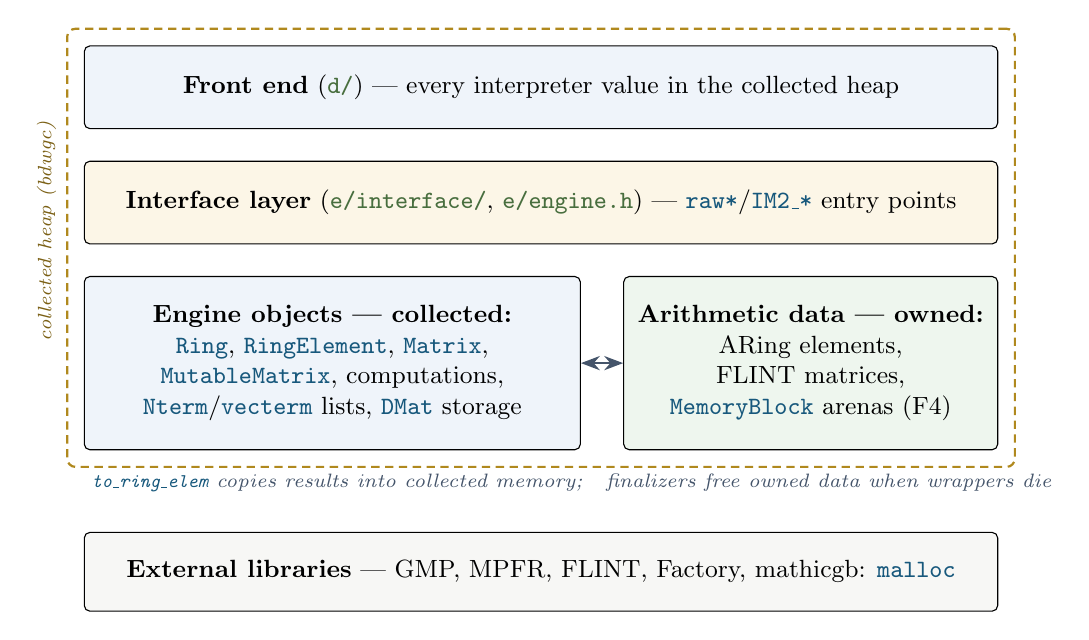
\begin{tikzpicture}[
  font=\small,
  zone/.style={draw, rounded corners=2pt, inner sep=5pt, align=center},
  lbl/.style={font=\scriptsize\itshape, text=m2slate},
  xarrow/.style={-{Stealth[length=2.4mm]}, thick, m2slate}
]
\node[zone, fill=boxblue, minimum width=11.6cm, minimum height=1.05cm] (fe)
  {\textbf{Front end} (\file{d/}) --- every interpreter value in the collected heap};
\node[zone, fill=boxamber, minimum width=11.6cm, minimum height=1.05cm, below=0.40cm of fe] (iface)
  {\textbf{Interface layer} (\file{e/interface/}, \file{e/engine.h}) --- \code{raw*}/\code{IM2\_*} entry points};
\node[zone, fill=boxblue, minimum width=6.3cm, minimum height=2.2cm, below=0.40cm of iface.south west, anchor=north west] (coregc)
  {\textbf{Engine objects --- collected:}\\
   \code{Ring}, \code{RingElement}, \code{Matrix},\\
   \code{MutableMatrix}, computations,\\
   \code{Nterm}/\code{vecterm} lists, \code{DMat} storage};
\node[zone, fill=boxgreen, minimum width=4.4cm, minimum height=2.2cm, below=0.40cm of iface.south east, anchor=north east] (coreown)
  {\textbf{Arithmetic data --- owned:}\\
   ARing elements,\\ FLINT matrices,\\
   \code{MemoryBlock} arenas (F4)};
\draw[{Stealth[length=2.4mm]}-{Stealth[length=2.4mm]}, thick, m2slate]
  (coregc.east) -- (coreown.west);
\node[lbl, align=center, yshift=-0.42cm] at ($(coregc.south)!0.5!(coreown.south)$)
  {\code{to\_ring\_elem} copies results into collected memory;\quad
   finalizers free owned data when wrappers die};
\node[zone, fill=codebg, minimum width=11.6cm, minimum height=1.0cm, below=3.65cm of iface] (libs)
  {\textbf{External libraries} --- GMP, MPFR, FLINT, Factory, mathicgb: \code{malloc}};
\begin{scope}[on background layer]
\node[draw=gcgold, densely dashed, thick, rounded corners=3pt,
      fit=(fe)(iface)(coregc), inner sep=6pt,
      label={[lbl, text=gcgold!70!black]178:{\rotatebox{90}{collected heap (bdwgc)}}}] {};
\end{scope}
\end{tikzpicture}
\captionof{figure}{Today: the collected heap (dashed) reaches through the
engine. Arithmetic data and external libraries already live outside it, with
copy-in and finalizer bridges at the seam.}
\label{fig:before}
\end{center}

\section{The life of a value: three walkthroughs}
\label{sec:life}

\begin{inbrief}
Three concrete stories --- a big integer at top level, an integer computed by
the engine, and a mutable matrix --- show the two memory worlds cooperating
in practice. The pattern is identical every time: \emph{work happens on
\code{malloc}'d data; the moment a value becomes visible to the front end,
its data is copied into collected memory and the original is freed.} The
system already knows exactly where its border is; it just crosses it in
hand-written, case-by-case ways.
\end{inbrief}

\subsection{An integer at top level: \code{n = 2\^{}100}}

The interpreter's big integers are GMP numbers, and the D source
(\file{d/gmp.d}) opens by describing its own two-world design:

\begin{quote}\itshape
``One type is mutable, and the vector of limbs gets allocated with the
standard memory allocator used by libgmp \ldots{} The other type is
immutable, and the limbs are allocated with libgc by us in [a] final step
after the computation.''
\end{quote}

\noindent So when the user computes $2^{100}$, the interpreter creates a
\emph{mutable} integer --- a GC-visible header whose limbs GMP puts on the
ordinary \code{malloc} heap --- and lets GMP arithmetic run at full speed
there. When the result is bound to \code{n}, \code{moveToZZ} performs the
border crossing: allocate an atomic GC block, \code{memcpy} the limbs into
it, repoint the header, and free the \code{malloc} original. The now-immutable
integer sits in a \code{ZZcell}, one arm of the interpreter's \code{Expr}
union (\file{d/parse.d} --- about forty variants: lists, hash tables,
strings, and one \code{Raw*Cell} arm per kind of engine object). From then
on the collector alone decides when $2^{100}$ dies.

\subsection{An integer computed by the engine}

Now let the \emph{engine} produce the number --- say an entry of a matrix
determinant over \code{ZZ}. The front end's \code{ZZ} is the legacy
\code{RingZZ} (\file{e/rings/ZZ.cpp}); its arithmetic allocates a GC header
with \code{malloc}'d limbs, computes with GMP, and then --- at the end of
essentially every operation --- calls \code{mpz\_reallocate\_limbs}
(\S\ref{sec:limbcopy}) so the result's limbs live in atomic GC memory
\emph{before} the value is wrapped in a \code{ring\_elem}. Engine integers
are, in the words of a comment in \file{e/interface/ringelement.cpp}, ``on
the `gc' side of the memory barrier, and \ldots{} read only'' --- which is
why handing one to the interpreter (\code{IM2\_RingElement\_to\_Integer},
reached from the D function \code{rawToInteger}) is a bare pointer copy, no
translation needed. The interpreter wraps that pointer in a \code{ZZcell}
and it becomes indistinguishable from a number the user typed.

Notice what this convention buys and costs. It buys safety-by-default: an
engine integer can \emph{always} be shown to the user, stored in a hash
table, or captured in a closure, because it is already collector-owned. It
costs a limb copy per arithmetic result --- even for the vast majority of
intermediate values that no user will ever see. The plan in
Chapter~\ref{ch:plan} moves that copy from ``every result'' to ``every
result that actually crosses'' --- which is precisely how the newer ARing
rings already behave (\S\ref{sec:border}).

\subsection{A mutable matrix, start to finish}

The richest story. The user asks for a random dense matrix over
$\mathbb{Z}/p$ and its rank:

\begin{enumerate}
\item The interpreter calls the interface layer's mutable-matrix
  entry points, in \file{e/interface/}; the ring's
  \code{ConcreteRing<ARingZZpFFPACK>} builds a
  \code{MutableMat<DMat<ARingZZpFFPACK>>} --- a garbage-collected wrapper
  (\code{MutableMatrix} is a \code{MutableEngineObject}, so it is
  GC-allocated \emph{and} finalized) that holds the dense matrix
  \emph{by value}.
\item The \code{DMat} inside allocates its element array --- and here is
  the surprise flagged in \S\ref{sec:census}: that array comes from
  \code{newarray}, i.e.\ \emph{scanned GC memory}, even though its entries
  here are plain \code{double}s. The interpreter meanwhile holds only a
  \code{RawMutableMatrixCell} --- a GC cell containing the wrapper pointer
  --- so the whole tower's lifetime hangs on interpreter reachability.
\item The rank computation dispatches through \code{MatrixOps}
  (\file{mat-linalg.hpp}) straight into FFLAS-FFPACK, which grinds on the raw element array with its own
  \code{malloc}'d temporaries. During the hot loop, the collector is
  irrelevant --- unless some \emph{other} thread allocates and triggers a
  collection, in which case this thread too is paused while the collector
  rescans, among everything else, the matrix array it never needed to look
  at.
\item The user moves on; the \code{RawMutableMatrixCell} becomes
  unreachable. At some later collection, the wrapper's finalizer runs
  (\file{e/finalize.cpp}), the \code{DMat} destructor clears each element
  and ``frees'' the array (a no-op, \S\ref{sec:wiring}); the memory
  returns to the heap at the sweep after that.
\end{enumerate}

\subsection{How deep the collector's roots go}

One more vignette, not about numbers at all, to calibrate how load-bearing
the collector is \emph{above} the engine: when a background task's handle
becomes unreachable, a finalizer on the task cell \emph{cancels the running
task} (\file{d/pthread.d}: ``cancelling inaccessible task \ldots{} still
running''). Garbage collection is not just an allocator here --- it is the
front end's lifetime-and-cleanup semantics, entangled with threads, foreign
functions, and user-visible behavior (\code{registerFinalizer} is a
documented language feature). This is why Chapter~\ref{ch:plan} proposes
\emph{confining} the collector rather than removing it: above the border it
is not overhead, it is the design.

\section{A census: who allocates where}
\label{sec:census}

\begin{inbrief}
Sorting the engine's data by memory regime shows a mostly clean pattern:
\emph{objects} (rings, matrices, computations) live in the collected heap;
\emph{arithmetic working data} (ARing elements, FLINT matrices, F4 scratch
monomials, everything inside the external libraries) lives outside it. The
collected side also holds the two linked-list term representations ---
polynomials (\code{Nterm}) and free-module vectors (\code{vecterm}) ---
which is where the collector and the cache both hurt, plus one genuine
surprise: the storage array inside \code{DMat}, the dense-matrix workhorse,
is itself collected memory. And exactly one coefficient ring ---
\code{CoefficientRingR}, Mike's ``wart'' --- computes \emph{in} the
collected heap.
\end{inbrief}

\subsection{The collected side}

Table~\ref{tab:gcside} lists the main engine residents of the collected
heap. The unifying fact: these are the objects the \emph{front end} can
hold, directly or indirectly, so their lifetimes are genuinely
session-shaped --- the collector is doing real work here.

\begin{table}[htbp]
\centering\small
\rowcolors{2}{gray!6}{white}
\begin{tabular}{@{}>{\raggedright\arraybackslash}p{0.25\textwidth}%
                  >{\raggedright\arraybackslash}p{0.27\textwidth}%
                  >{\raggedright\arraybackslash}p{0.37\textwidth}@{}}
\toprule
\textbf{What} & \textbf{Where} & \textbf{Memory shape} \\
\midrule
\code{Ring} and subclasses & \file{e/rings/ring.hpp} &
  GC object, auto-finalized (via \code{MutableEngineObject}) \\
\code{RingElement} & \file{e/ring-elements/} &
  GC object: a \code{Ring*} plus a \code{ring\_elem} \\
\code{Matrix} (immutable) & \file{e/matrices/} &
  GC object: \code{gc\_vector} of columns, each a \code{vecterm} list \\
\code{MutableMatrix} & \file{e/basic-mutable-\linebreak matrices/} &
  GC wrapper (finalized) over a dense/sparse implementation \\
\code{FreeModule}, \code{MonomialIdeal}, \code{SchreyerOrder} &
  \file{e/free-modules/}, \file{e/monomials/} & GC objects \\
\code{Computation} family (GB, resolutions, \ldots) &
  \file{e/computations/} & GC objects, finalized \\
Polynomial terms (\code{Nterm}) & \file{e/rings/ringelem.hpp} &
  hand-allocated \emph{scanned} GC nodes, exponents inline \\
Vector terms (\code{vecterm}) & \file{e/rings/ringelem.hpp} &
  GC list nodes (with the in-tree TODO of \S\ref{sec:optin}) \\
Standalone monomials & \file{e/monomials/monoid.cpp} &
  \emph{atomic} GC arrays (\code{newarray\_atomic}) \\
\bottomrule
\end{tabular}
\caption{Principal engine residents of the collected heap today.}
\label{tab:gcside}
\end{table}

Two structural notes on this table. First, polynomials and matrix columns
are \emph{per-term allocations}: a polynomial with a million terms is a
million separate scanned GC blocks chained by pointers. Every collection
re-walks the chain; every traversal hops the heap. This one row is most of
the performance story of \S\ref{sec:costs}. Second, \code{Nterm} nodes must
be scanned (their \code{coeff} may point at collected data), so they cannot
even use the cheaper atomic allocation --- the representation forces the
collector's most expensive treatment.

\subsection{The owned side}

The modern coefficient rings --- the \emph{ARings}, in
\file{e/basic-rings/} --- are where the engine already practices what
Chapter~\ref{ch:plan} preaches. An ARing is a plain C++ class satisfying an
informal contract (spelled out by the base class \code{SimpleARing} and the
worked example \code{DummyRing} in \file{aring.hpp}): a plain-data
\code{ElementType}; GMP-style lifetime methods \code{init},
\code{init\_set}, \code{set}, and a \emph{static} \code{clear}; the
arithmetic (\code{add}, \code{mult}, \code{invert}, \ldots); conversions
\code{to\_ring\_elem}/\code{from\_ring\_elem} (\S\ref{sec:border}); and
\code{promote}/\code{lift}/\code{eval} for moving between rings. Each ARing
also carries a tag in the (plain, non-\code{class}) \code{enum RingID} used
for dispatch --- with a sentinel \code{ring\_old} meaning ``any ring that is
not one of these.'' The contract even includes RAII helpers --- a nested
\code{Element} whose constructor calls \code{init} and whose destructor
calls \code{clear}, and an \code{ElementArray} --- so scoped, non-collected
element lifetimes are already idiomatic. A dedicated unit-test harness
exercises all of it (\file{e/unit-tests/ARingTest.hpp}), and the convenience
wrapper Mike remembered at the meeting (``you give it the ring and an
element \ldots{} then you can call \code{operator+}'') exists twice: as
\code{RingElem} (\file{e/unit-tests/RingElem.hpp}, over the virtual
\code{Ring} interface) and as the RAII-only \code{ARingElement<RT>}
(\file{e/SLP/SLP-imp.hpp}) --- a duplication \S\ref{sec:ws-aring} proposes
to unify.

Crucially, every ARing's \emph{working element} lives outside the collected
heap (Table~\ref{tab:arings}) --- with the single exception of
\S\ref{sec:wart}.

\begin{table}[htbp]
\centering\small
\rowcolors{2}{gray!6}{white}
\begin{tabular}{@{}llll@{}}
\toprule
\textbf{Ring} & \textbf{Class} & \textbf{ElementType} & \textbf{Working memory} \\
\midrule
$\mathbb{Z}$ & \code{ARingZZGMP} & \code{\_\_mpz\_struct} & \code{malloc} (GMP limbs) \\
$\mathbb{Z}$ & \code{ARingZZ} & \code{fmpz} & \code{malloc} (FLINT) \\
$\mathbb{Q}$ & \code{ARingQQGMP} & \code{\_\_mpq\_struct} & \code{malloc} (GMP) \\
$\mathbb{Q}$ & \code{ARingQQFlint} & \code{fmpq} & \code{malloc} (FLINT) \\
$\mathbb{Z}/p$ & \code{ARingZZp} & \code{int} & none (log tables) \\
$\mathbb{Z}/p$ & \code{ARingZZpFFPACK} & \code{double} & none (value) \\
$\mathbb{Z}/p$ & \code{ARingZZpFlint} & \code{mp\_limb\_t} & none (value) \\
$\mathrm{GF}(p^n)$ & \code{ARingGFM2} & \code{int} & none (log tables) \\
$\mathrm{GF}(p^n)$ & \code{ARingGFFlint(Big)} & \code{fq\_zech}/\code{fq\_nmod} & \code{malloc} (FLINT) \\
$\mathbb{R}$, $\mathbb{C}$ (machine) & \code{ARingRR}, \code{ARingCC} & \code{double}(s) & none (value) \\
$\mathbb{R}$, $\mathbb{C}$ (mpfr) & \code{ARingRRR}, \code{ARingCCC} & \code{\_\_mpfr\_struct}(s) & \code{malloc} (MPFR) \\
intervals & \code{ARingRRi}, \code{ARingCCi} & \code{\_\_mpfi\_struct}(s) & \code{malloc} (MPFI) \\
any legacy ring & \code{CoefficientRingR} & \code{ring\_elem} & \emph{collected heap} (\S\ref{sec:wart}) \\
\bottomrule
\end{tabular}
\caption{The coefficient-ring census (\file{e/basic-rings/}, plus the
adapter in \file{e/coeffrings.hpp}). Working elements are \code{malloc}'d
or plain values everywhere --- except the last row.
(\code{ARingTower}, experimental, mixes regimes and is omitted.)}
\label{tab:arings}
\end{table}

The glue between the two ring generations is
\code{ConcreteRing<RingType>}, in \file{aring-glue.hpp}: a subclass of the
virtual \code{Ring} interface that owns its ARing by --- note the type ---
a \code{std::unique\_ptr}, and implements every \code{Ring} virtual by
unwrapping \code{ring\_elem}s into ARing elements, computing, and
re-wrapping. The ownership idiom of Chapter~\ref{ch:plan} is already in
the tree.

Beyond the ARings, the engine's highest-performance kernels already manage
their own memory wholesale: the F4 Gr\"obner engine, the noncommutative
F4, the newer \file{gb-f4/}, and the Schreyer-resolution code all stage
their monomial and coefficient data in \code{MemoryBlock} arenas ---
memtailor's \code{memt::Arena} under a thin wrapper
(\file{e/MemoryBlock.hpp}), allocated with plain \code{operator new[]},
invisible to the collector, and released all at once when the computation
ends. The external libraries (GMP, MPFR, FLINT, Factory, mathicgb) likewise
\code{malloc} everything. In other words: \emph{the pattern
Chapter~\ref{ch:plan} proposes is already how the fastest code in the
engine works.} The plan's job is to make it the rule rather than the
exception, and to give it a policed border.

(A naming hazard for anyone reading the F4 sources: the classic F4 engine
also has an \code{F4MemoryBlock} --- which, despite the similar name, is a
GC-allocated slab type. Two arena abstractions with opposite memory regimes
coexist; \S\ref{sec:ws-border} standardizes on the non-collected one.)

\subsection{The dense-matrix surprise}
\label{sec:dmatsurprise}

\code{DMat<ARing>} (\file{e/basic-mutable-matrices/dmat.hpp}) is the dense
matrix the linear-algebra stack computes on. Its kernels are exemplarily
GC-free: \code{MatrixOps} dispatches by coefficient ring to FFLAS-FFPACK,
FLINT, LAPACK, or Eigen, all of which treat the element array as a raw
buffer. But the element array \emph{itself} is allocated with
\code{newarray} --- scanned, collected memory --- and the destructor
dutifully \code{clear}s each element and calls the no-op \code{freemem}.
Why scanned? Because a \code{DMat}'s elements are sometimes \emph{GC
handles}: the adapter ring of \S\ref{sec:wart} stores \code{ring\_elem}s
directly in the array, and scanning is the only thing keeping those alive.
So the one GC-backed coefficient ring forces the collector into every dense
matrix's storage, whatever the coefficients. (The FLINT-backed
specializations of \code{DMat} instead hold native \code{malloc}'d FLINT
matrices --- accompanied by a frank comment in
\file{dmat-zz-flint.hpp}: ``objects of this class should \emph{not} go to
the front end \ldots{} \code{fmpz\_t}'s might be garbage collected out from
under you.'') Mike's request that ``all DMAT-type computations'' be
GC-free is thus two small steps from true, and \S\ref{sec:ws-matrix} takes
them.

\subsection{The one exception: \code{CoefficientRingR}}
\label{sec:wart}

The wart Mike described at the meeting --- ``all of a sudden, there's one
A-ring type that is garbage collected, none of the other ones are'' --- is
\code{CoefficientRingR} (\file{e/coeffrings.hpp}). It is the adapter that
lets \emph{any} legacy ring (a fraction field, a quotient ring, anything
tagged \code{ring\_old}) play the role of an ARing, and it does so by the
simplest possible trick: its \code{ElementType} \emph{is} \code{ring\_elem}.
Its lifetime methods say everything:

\begin{lstlisting}
void init(elem &result)  const { result = R->zero(); }
void clear(elem &result) const { (void) result; }   // no-op: the collector owns it
void to_ring_elem(ring_elem &result, const elem &a)   const { result = a; }
void from_ring_elem(elem &result, const ring_elem &a) const { result = a; }
\end{lstlisting}

\noindent \code{clear} frees nothing because there is nothing it may free:
the elements are collected objects belonging to the legacy ring.
Conversions are pointer copies; the ``border'' is a door standing open.
Any legacy ring acquires this adapter on demand
(\code{Ring::getCoefficientRingR()}), and the F4 vector-arithmetic layer
selects it for old non-prime-field coefficients --- announcing itself with
a stray diagnostic, \code{"Using GC ring in VectorArithmetic."}, that ships
to \code{stdout} today.

This also resolves the puzzle Mike voiced (``it seems to work mostly okay
\ldots{} but I don't know exactly why that would be the case''): it works
\emph{because} the containers that hold these elements --- \code{DMat}'s
scanned array (\S\ref{sec:dmatsurprise}), the GC-backed
\code{ElementArray} this ring supplies --- are visible to the collector, so
reachability flows through them. The arrangement is internally consistent;
its price is that it globally couples container memory to the collector.
Unpicking that coupling --- without breaking fraction-field coefficients
--- is Workstream~3 (\S\ref{sec:ws-aring}).

\section{The border crossings today}
\label{sec:border}

\begin{inbrief}
Data crosses between the two memory worlds at two kinds of checkpoint,
both already established: \emph{numbers} cross by having their digits
copied into (atomic) collected memory --- the \code{to\_ring\_elem} /
\code{mpz\_reallocate\_limbs} pattern --- and \emph{owned resources} are
tied to collected wrappers by \emph{finalizers} registered in
\file{e/finalize.cpp}. Both mechanisms work; both have accumulated
inconsistencies worth cleaning up during the migration.
\end{inbrief}

\subsection{Crossing by copy: numbers}
\label{sec:limbcopy}

When arithmetic done outside the collected heap produces a result the front
end must hold, the engine does not hand over the \code{malloc}'d object ---
it copies the number's digits (GMP's \emph{limbs}) into atomic GC memory
and releases the original. The helpers live in
\file{e/interface/gmp-util.h}; the integer case, condensed:

\begin{lstlisting}
mp_limb_t* p = (mp_limb_t*) getmem_atomic(n * sizeof(mp_limb_t));
memcpy(p, z->_mp_d, n * sizeof(mp_limb_t));
mpz_clear(z);          // free the malloc'd original
z->_mp_d = p;          // repoint at the GC-heap copy
\end{lstlisting}

\noindent with siblings for rationals, reals, intervals, and complexes
(\code{moveTo\_gmpQQ}, \code{moveTo\_gmpRR}, \code{moveTo\_gmpRRi},
\code{moveTo\_gmpCC}). The copied limbs are \emph{atomic} memory: the
collector keeps them alive but never scans them --- numbers cannot contain
pointers, and this is the promise that makes big-number data cheap for the
collector to hold.

\subsection{Crossing by conversion: the ARing pattern}
\label{sec:aringborder}

The ARings institutionalize the same copy into a named pair of methods.
Inside a computation, elements are the ring's native \code{ElementType}
(a FLINT \code{fmpz}, a \code{double}, \ldots) on \code{malloc} or in
registers; \code{to\_ring\_elem} is the checkpoint where a value becomes a
front-end-safe \code{ring\_elem}. The FLINT integers show the full ritual
(\file{e/basic-rings/aring-ZZ-flint.hpp}):

\begin{lstlisting}
void to_ring_elem(ring_elem& result, const ElementType& a) const
{
  mpz_ptr b = getmemstructtype(mpz_ptr);  // GC-heap mpz header
  mpz_init(b);                            // malloc'd limbs, briefly
  fmpz_get_mpz(b, &a);                    // decode the FLINT value
  mpz_reallocate_limbs(b);                // copy limbs into atomic GC memory
  result = ring_elem(b);
}
void from_ring_elem(ElementType& result, const ring_elem& a) const
{
  fmpz_set_mpz(&result, a.get_mpz());     // copy back out into FLINT
}
\end{lstlisting}

\noindent Nothing FLINT-encoded ever touches the collected heap; nothing
collected is ever handed to FLINT. Each ring pays this toll only when a
value actually crosses --- which is the entire performance thesis of
Chapter~\ref{ch:plan} in two functions. The one ring that skips the toll
booth is \code{CoefficientRingR} (\S\ref{sec:wart}), whose conversions are
pointer copies because its elements never left the collected heap in the
first place.

\subsection{Crossing by finalizer: owned resources}
\label{sec:finalizers}

The reverse bridge ties \code{malloc}-world resources to the lifetime of a
collected object. \file{e/finalize.cpp} is the registry: its
\code{intern\_*} functions register a collector finalizer on the wrapper,
and when the wrapper becomes unreachable the finalizer releases what the
collector cannot see.

\begin{table}[htbp]
\centering\small
\rowcolors{2}{gray!6}{white}
\begin{tabular}{@{}lll@{}}
\toprule
\textbf{Class (registered by \code{intern\_*})} & \textbf{Variant} & \textbf{On death} \\
\midrule
\code{MonomialIdeal} & plain & \code{remove\_MonomialIdeal()} \\
\code{GBComputation} & ignore-self & \code{remove\_gb()} \\
\code{ResolutionComputation} & plain & \code{delete G} \\
\code{SchreyerOrder} & plain & \code{remove()} \\
\code{MutableMatrix} & plain & explicit destructor call \\
\bottomrule
\end{tabular}
\caption{The finalizer registry in \file{e/finalize.cpp}. (The front end
registers its own finalizers separately, for task cells, mutexes, and
foreign-function handles.)}
\label{tab:finalizers}
\end{table}

Three inconsistencies in this table are worth naming, because
Phase~1 of the plan (\S\ref{sec:roadmap}) tidies exactly these:

\begin{itemize}
\item \textbf{Double registration.} Every \code{MutableEngineObject}
  \emph{already} received a finalizer at construction (from
  \code{our\_gc\_cleanup}, \S\ref{sec:optin}); the \code{intern\_*} call
  then \emph{replaces} it. The code knows this --- \code{intern\_polyring}
  is a documented no-op for precisely that reason --- but the two-layer
  scheme is easy to misread and easy to get wrong when adding a class.
\item \textbf{Mixed variants.} One class registers with the ignore-self
  variant, four with the plain one; the difference (whether a
  self-referential object can ever be collected) is subtle enough that it
  should be a policy, not an accident.
\item \textbf{Mixed teardown styles.} One finalizer calls \code{delete},
  one calls a destructor explicitly without deallocating, three call
  bespoke \code{remove} methods. With rule-of-five engine types
  (\S\ref{sec:ownership}), all of these collapse into ``destroy the owned
  object.''
\end{itemize}

One more detail for completeness: the allocator itself anticipates
finalizers misbehaving --- \code{getmem} carries a thread-local reentrancy
guard with a comment noting that finalizers may legitimately allocate
during collection. The plan's finalizer policy (\S\ref{sec:finalizerpolicy})
forbids relying on that legitimacy; \S\ref{sec:flintwall} shows why.

\section{What the current arrangement costs}
\label{sec:costs}

\begin{inbrief}
Four costs, in descending order of pain: collector time stolen from
computations (Mike's estimate has grown from ``about 20\%'' to ``sometimes a
multiple-times hit''); cache-hostile linked-list representations that the
collector makes both possible and expensive; memory held longer than
necessary by conservative scanning in a heap that can never compact; and a
hard wall that keeps FLINT's fast integers and rationals from becoming the
defaults. None of these are new observations --- the tree itself is
annotated with comments wishing parts of it were not collected.
\end{inbrief}

\subsection{Time}

The collector charges computations in three ways. First, collections are
triggered by allocation volume, and the engine's classic representations
allocate \emph{per term}: a long polynomial multiplication churns out
millions of \code{Nterm} nodes, each a separate collected block, so hot
loops are exactly the code that summons the collector most often. Second,
each collection stops every thread and re-marks the live heap --- and the
cost of marking is proportional to \emph{scanned} live memory, which
(\S\ref{sec:census}) includes every term node of every polynomial a session
still holds, plus every dense matrix's element array. A computation pays
rent on data it never touches. Third, Macaulay2 runs the collector in plain
stop-the-world mode (\S\ref{sec:wiring}); nothing is incremental, so pauses
land in full.

How much does this cost end to end? Mike's testimony at the meeting: ``I
used to think it was \ldots{} like a 20\% hit \ldots{} I would say sometimes
it's a multiple[-]times hit \ldots{} it spends too much time in garbage
collection,'' together with the converse experience that removing the
collector from a computation type ``speeds things way up.'' These are
recollections, not benchmarks --- which is precisely why Phase~0 of the
plan (\S\ref{sec:roadmap}) begins by measuring collector share on a fixed
suite, so every later phase can report a before/after number.

\subsection{Cache}

A linked-list polynomial is a pointer chase: each term is a separate heap
block, adjacent terms need not be adjacent in memory, and every term visit
risks a cache miss. As Mike put it, linked lists ``just do[]n't play well
with cache.'' The collected heap deepens the problem --- allocation order
interleaves unrelated data, and a non-moving collector can never migrate a
polynomial's terms back together. The contrast already exists in-tree: the
noncommutative-algebra code (with Frank Moore) stores a polynomial as a
coefficient array plus one flat integer array of all its monomials
(\code{Polynomial<T>} in \file{e/Polynomial.hpp}) --- the
``couple [of] arrays'' shape Mike sketched at the meeting. Workstream~5
(\S\ref{sec:ws-poly}) builds on exactly that precedent.

\subsection{Retention and fragmentation}

Conservative scanning keeps anything that \emph{looks} reachable: an
unlucky integer on some stack pins a dead matrix, and everything the matrix
references, until the coincidence passes (\S\ref{sec:boehm}). Since the
heap never compacts, long sessions fragment; and since the runtime pre-grows
the heap aggressively (150\,MB+ at startup, \S\ref{sec:wiring}) and
collects by heap-growth heuristics, a Macaulay2 process holds
substantially more memory than its live data. At top level this is a fair
trade for never thinking about lifetimes. Inside a computation it is pure
overhead.

\subsection{The FLINT wall}
\label{sec:flintwall}

FLINT's integer type \code{fmpz} is one machine word that plays exactly the
kind of game a conservative collector cannot referee: small values are
stored \emph{in} the word, and large values store a \emph{transformed}
pointer to a heap structure --- shifted and tagged, so the true address
never appears in memory as itself. To the collector (\S\ref{sec:boehm}),
a large \code{fmpz} is a disguised pointer: invisible, hence dead, hence
reclaimable out from under the computation. FLINT values are therefore
banned from the collected heap --- a fact the tree states plainly in the
FLINT-matrix warning quoted in \S\ref{sec:dmatsurprise}.

The consequence Mike lamented at the meeting: the FLINT integers and
rationals --- ``the ones that are default \ldots{} should be [ZZ and QQ],
but they're not'' --- exist as dormant ARings. Today's front-end \code{ZZ}
is the legacy GMP-based \code{RingZZ} (not an ARing at all), today's
\code{QQ} is the GMP ARing \code{ARingQQGMP}, and the FLINT versions are
reachable only through developer functions (\code{rawARingZZFlint},
\code{rawARingQQFlint}). Making them the defaults requires nothing more
--- and nothing less --- than a border that always copies
(\S\ref{sec:ws-flint}).

\begin{warstory}
It was once tried the other way: FLINT had a mode (\code{FLINT\_USES\_GC})
for cooperating with a collector by keeping a side array of every GMP
number in use, registered as a GC root. Mike, at the meeting, on how that
went: the side array was modified \emph{inside} finalization --- freeing
one number triggered finalizers that freed others, which rewrote the very
array being traversed --- ``it wasn't done in a way \ldots{} where you
could alias this list. So it just didn't work at all.'' He called the
resulting bug ``a hellhole \ldots{} one of the worst bugs. It took me
forever to find.'' Without finalization the scheme limped along; with
finalization it collapsed. The lesson, encoded in the finalizer policy of
\S\ref{sec:finalizerpolicy}: never let finalizers mutate shared registries,
and never try to make a foreign library's \code{malloc} world
collector-visible by bookkeeping. Copy at the border instead.
\end{warstory}

\section{The seam is already half-built}
\label{sec:seam}

Chapter~\ref{ch:plan} will read as less radical if this chapter's findings
are stacked up in one place. The engine already has: a named conversion
ritual at the number border (\code{to\_ring\_elem} /
\code{mpz\_reallocate\_limbs}, \S\ref{sec:border}); a coefficient-ring
contract with GMP-style \code{init}/\code{clear} lifetimes and RAII
helpers, satisfied by every coefficient ring but one with working memory
already outside the collector (\S\ref{sec:census}); a glue class that owns its ring
through \code{std::unique\_ptr} (\file{aring-glue.hpp}); GC-free
linear-algebra kernels; arena allocators in its hottest Gr\"obner code; a
single finalizer registry (\file{e/finalize.cpp}); and a flattened
polynomial representation in production use. It even has the opinions: the
tree is dotted with comments like ``\code{TODO: why is this garbage
collected?}'' (\file{e/rings/ringelem.hpp}) and ``\code{TODO: make sure
monoid is deconstructed and not garbage collected}''
(\file{e/monoid.hpp}).

What it does not have is a \emph{policed} border: \code{DMat} storage sits
in the collected heap for the sake of one adapter ring; the legacy
\code{ZZ} pays a limb copy on every intermediate result; finalizers are
registered in two layers with three teardown styles; and nothing stops a
new engine file from quietly including \file{newdelete.hpp}. Turning this
half-built seam into an enforced architecture is what the next chapter
proposes.

% ---------------- chapter 2 ----------------
\chapter{A Plan for Confining the Collector}
\label{ch:plan}
\begin{inbrief}
The plan is to \emph{confine} the collector, not remove it. The front end
keeps garbage collection forever. The engine's computational core ---
ARing arithmetic, dense-matrix work, and eventually the classic
polynomial/matrix types --- moves to ordinary C++ ownership
(\code{std::unique\_ptr}, references, RAII), which it is already halfway to
using. The only place engine code may touch collected memory is the interface
layer, where results are \emph{copied} into the collector's heap for the front
end. The migration proceeds in six phases, each independently shippable and
testable, ordered so that the riskiest changes come after the mechanical ones
have hardened the border. Cross-cutting rules --- ownership conventions,
a finalizer policy, and CI enforcement --- keep the two memory worlds from
bleeding into each other again.
\end{inbrief}

\section{What Mike asked for}
\label{sec:asked}

Chapter~\ref{ch:current} described the machine as it is. This chapter answers
the specific requests Mike made at the July 2026 engine meeting (collected
with timestamps in \file{src/mike-requests.md}). The two governing quotes:

\begin{mikesays}[on the goal]
``If you could give us a roadmap on how to get rid of the garbage collector
\ldots'' --- and immediately sharpened: ``So, it's \emph{not} to get rid of
the garbage collector. The garbage collector \ldots{} should be set up only
for things in the interface directory.''
\end{mikesays}

\begin{mikesays}[on the deliverable]
A proposal document --- not a giant pull request --- ``detailed enough for
\ldots{} an overview for us to follow, and detailed enough for \ldots{} Opus
or one of the lesser agents later to follow, and then we can edit the
proposal.''
\end{mikesays}

Table~\ref{tab:requests} maps every actionable request from the meeting to
the part of this chapter that addresses it. Nothing Mike asked for is
silently dropped; two items he himself labeled speculative are treated as
optional investigations rather than plan commitments.

\begin{table}[htbp]
\centering\small
\rowcolors{2}{gray!6}{white}
\begin{tabular}{@{}p{0.56\textwidth}l@{}}
\toprule
\textbf{Request (from \file{mike-requests.md})} & \textbf{Addressed in} \\
\midrule
Roadmap document, editable, executable in supervised steps
  & this chapter; \S\ref{sec:roadmap} \\
GC restricted to the interface directory / front-end objects
  & \S\ref{sec:target}, \S\ref{sec:ws-border} \\
All ARing computations free of GC
  & \S\ref{sec:ws-aring} \\
All DMat-type (dense linear algebra) computations free of GC
  & \S\ref{sec:ws-matrix} \\
Split \code{Matrix} into a GC'd front-end type and an engine-only owned type,
with conversions both ways
  & \S\ref{sec:ws-matrix} \\
Rust-style ownership (\code{unique\_ptr} owns; references borrow)
  & \S\ref{sec:groundrules} \\
Keep/clean up finalization for objects wrapping non-GC memory
  & \S\ref{sec:groundrules}, \S\ref{sec:ws-border} \\
Fix the one garbage-collected ARing (the coefficient-ring wart)
  & \S\ref{sec:ws-aring} \\
(Adjacent) cache-friendly, non-linked-list polynomials
  & \S\ref{sec:ws-poly} \\
(Adjacent) more FLINT rings; FLINT \code{ZZ}/\code{QQ} as defaults;
optionally teach the collector about FLINT's encoding
  & \S\ref{sec:ws-flint} \\
\bottomrule
\end{tabular}
\caption{Every request from the July meeting, and where this plan answers it.}
\label{tab:requests}
\end{table}

\section{The target architecture: three zones and one rule}
\label{sec:target}

Today the collected heap reaches all the way down through the engine
(Figure~\ref{fig:before}, page~\pageref{fig:before}). The end state confines
it to the top of the picture:

\begin{center}
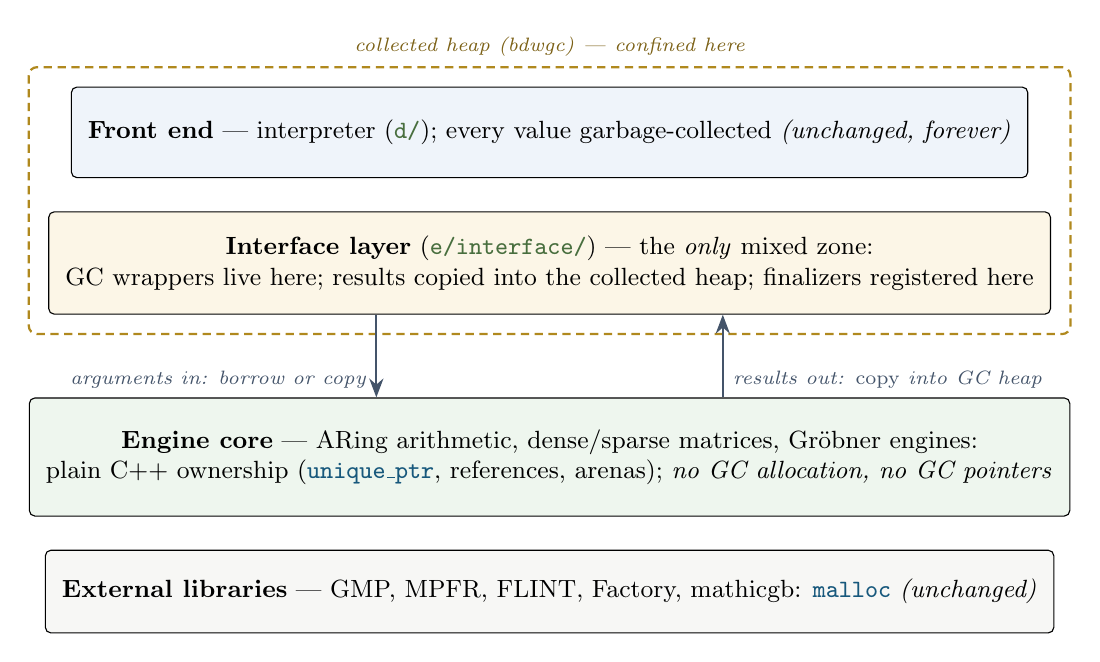
\begin{tikzpicture}[
  font=\small,
  zone/.style={draw, rounded corners=2pt, minimum width=11.6cm, inner sep=6pt, align=center},
  lbl/.style={font=\scriptsize\itshape, text=m2slate},
  xarrow/.style={-{Stealth[length=2.4mm]}, thick, m2slate}
]
\node[zone, fill=boxblue,  minimum height=1.15cm] (fe)
  {\textbf{Front end} --- interpreter (\file{d/}); every value garbage-collected \emph{(unchanged, forever)}};
\node[zone, fill=boxamber, minimum height=1.3cm, below=0.42cm of fe] (iface)
  {\textbf{Interface layer} (\file{e/interface/}) --- the \emph{only} mixed zone:\\
   GC wrappers live here; results copied into the collected heap; finalizers registered here};
\node[zone, fill=boxgreen, minimum height=1.5cm, below=1.05cm of iface] (core)
  {\textbf{Engine core} --- ARing arithmetic, dense/sparse matrices, Gr\"obner engines:\\
   plain C++ ownership (\code{unique\_ptr}, references, arenas); \emph{no GC allocation, no GC pointers}};
\node[zone, fill=codebg,  minimum height=1.05cm, below=0.42cm of core] (libs)
  {\textbf{External libraries} --- GMP, MPFR, FLINT, Factory, mathicgb: \code{malloc} \emph{(unchanged)}};
\draw[xarrow] ([xshift=-2.2cm]iface.south) -- ([xshift=-2.2cm]core.north)
  node[pos=0.78, left, lbl] {arguments in: borrow or copy};
\draw[xarrow] ([xshift=2.2cm]core.north) -- ([xshift=2.2cm]iface.south)
  node[pos=0.22, right, lbl] {results out: \emph{copy} into GC heap};
\begin{scope}[on background layer]
\node[draw=gcgold, densely dashed, thick, rounded corners=3pt,
      fit=(fe)(iface), inner sep=7pt, label={[lbl, text=gcgold!70!black]90:collected heap (bdwgc) --- confined here}] {};
\end{scope}
\end{tikzpicture}
\captionof{figure}{The target: the collector's reach ends at the interface layer.}
\label{fig:after}
\end{center}

Everything in this chapter serves one rule:

\begin{center}
\begin{minipage}{0.88\textwidth}
\centering\itshape
Engine-core code neither allocates from the collected heap nor stores
pointers into it. Whatever crosses the border is copied, at the border, by
interface-layer code.
\end{minipage}
\end{center}

Three honest qualifications, so the rule is a plan and not a slogan:

\begin{itemize}
\item \textbf{The rule is the end state, reached subsystem by subsystem.} The
  linear-algebra pipeline (ARings, \code{DMat}, mutable matrices) gets there
  first because it is nearly there already; the Gr\"obner engines follow; the
  classic term-list world (\code{Nterm}/\code{vecterm} polynomials and the
  immutable \code{Matrix} built from them) goes last --- and parts of it may
  be \emph{replaced} (\S\ref{sec:ws-poly}) rather than converted, because
  migrating a linked-list representation the collector was hiding is exactly
  when to reconsider the representation itself.
\item \textbf{``Copy at the border'' is a feature, not a compromise.} Border
  crossings are rare relative to the arithmetic between them, and the engine
  \emph{already} pays for exactly this copy where it matters --- the ARing
  conversion functions copy number data into collected memory today
  (\S\ref{sec:border}). The plan generalizes an existing, proven pattern
  rather than inventing a new one.
\item \textbf{The front end and the external libraries do not change at all.}
  The collector stays; \code{malloc} stays; only the territory between them is
  renegotiated.
\end{itemize}

\section{Ground rules for the whole migration}
\label{sec:groundrules}

These conventions apply to every workstream and phase below. They are the
answer to Mike's ``managed kind of like you would manage Rust objects,'' made
specific enough to enforce.

\subsection{Ownership conventions}
\label{sec:ownership}

\begin{center}
\small
\begin{tabular}{@{}lll@{}}
\toprule
\textbf{Relationship} & \textbf{Rust} & \textbf{Engine-core C++} \\
\midrule
I own it, exclusively & \code{Box<T>} / value & value member or \code{std::unique\_ptr<T>} \\
I am lending it to you & \code{\&T} / \code{\&mut T} & \code{const T\&} / \code{T\&} \\
I am giving it to you & move & pass/return by value (move semantics) \\
Many owners & \code{Rc<T>} (rare) & \code{std::shared\_ptr<T>} --- \emph{requires justification} \\
Raw owning pointer & forbidden & forbidden \\
\bottomrule
\end{tabular}
\end{center}

Concretely: engine-core classes get real destructors, copy/move constructors,
and \code{=\,delete} where copying is wrong --- ordinary rule-of-five C++.
Functions take \code{const\&} for inputs, \code{\&} for in-place outputs, and
return results by value. A raw pointer in engine-core code always means
``borrowed, non-null unless documented, never freed by the holder.'' None of
this is exotic; it is what the ARing element contract already does by hand
with \code{init}/\code{clear} pairs, upgraded from convention to type system
where possible.

\subsection{Finalizer policy}
\label{sec:finalizerpolicy}

Finalizers remain --- but only on border-layer wrapper objects, only
registered through one auditable registry (today's \code{intern\_*} machinery
in \file{e/finalize.cpp}, consolidated in Phase~1), and only with bodies that
are boring on purpose:

\begin{enumerate}
\item A finalizer may release resources owned by \emph{its own} object
  (typically by \code{delete}-ing the engine-core object a wrapper owns ---
  which, with rule-of-five types, frees everything underneath via ordinary
  destructors).
\item A finalizer must not allocate, must not touch the collected heap, must
  not take locks shared with allocation paths, and must not modify any global
  registry that other finalizers also modify.
\item Every class that registers finalizers is listed in one place, so the
  full set is auditable at a glance.
\end{enumerate}

Rule 2 is written in blood; \S\ref{sec:flintwall}'s cautionary tale (the old
\code{FLINT\_USES\_GC} side-array corrupting itself when finalizers fired
during collection) is precisely what it forbids.

\subsection{Mechanical enforcement}
\label{sec:enforcement}

Conventions decay unless a machine checks them. Three cheap checks, added in
Phase~1 and kept forever:

\begin{itemize}
\item \textbf{Include hygiene in CI.} Engine-core sources (a growing explicit
  list, eventually ``all of \file{e/} outside \file{e/interface/}'') must not
  include \file{newdelete.hpp}, \file{gc-include.h}, or any \file{gc/*}
  header, and must not mention \code{GC\_}, \code{getmem}, or
  \code{our\_new\_delete}. A grep in CI fails the build with a pointer to this
  document. Files not yet migrated stay off the list --- so the check never
  blocks unrelated work, and progress is literally the list growing.
\item \textbf{Sanitizer builds.} Once a subsystem is GC-free, it can finally
  run under AddressSanitizer and LeakSanitizer in CI (the collector currently
  drowns both in noise). Leaks in migrated code become test failures instead
  of folklore. This is a fringe benefit of the whole project worth naming: we
  get modern memory tooling back.
\item \textbf{Border-crossing counters (debug builds).} The interface layer
  counts copies in and out per type. A hot loop accidentally crossing the
  border on every iteration shows up as a number, not a mystery slowdown.
\end{itemize}

\subsection{Tests first, measurements always}
\label{sec:testsfirst}

Mike's instinct at the meeting --- put unit tests ``way up above'' in the
checklist and work test-driven --- is adopted as policy: no phase changes
behavior before it has tests pinning the current behavior. The existing ARing
unit-test harness (\S\ref{sec:census}) is the model. Each phase in
\S\ref{sec:roadmap} names its acceptance tests. And every phase begins and
ends with the same benchmark suite (fixed in Phase~0), reporting wall time
and collector share, so ``it speeds things way up'' becomes a measured
number per phase rather than an impression.

\section{Workstream 1: harden the border}
\label{sec:ws-border}

\begin{mikesays}[on finalization]
``You tell the garbage collector, hey, when this one goes out of scope, I
want you to call this other function \ldots{} typically it's on a per-class
basis, for real.'' And on the state of that global picture: it is
``a global piece of information that is hard to get cracked.''
\end{mikesays}

\textbf{Where we are.} The border exists but is unpoliced
(\S\ref{sec:seam}): finalizers are registered in two layers with three
teardown styles (\S\ref{sec:finalizers}); the GC surface is enumerable
(\file{e/engine.h} plus \file{e/interface/*.h}) but nowhere enumerated; and
nothing prevents new engine code from allocating collected memory.

\textbf{The change.}
\begin{enumerate}
\item \textbf{Make ``the interface directory'' literally true.} Relocate
  \file{e/finalize.cpp}/\file{.hpp} into \file{e/interface/}, and write the
  one-page description of the GC surface: which headers, which types, which
  \code{raw*} functions may traffic in collected pointers. Mike's phrase
  becomes a checkable property of the tree.
\item \textbf{One finalizer mechanism.} Collapse the double registration of
  \S\ref{sec:finalizers}: pick a single registration site (the
  \code{intern\_*} registry), a single variant (uniform ignore-self unless
  the Phase-1 audit finds a real cross-object cycle), and a single teardown
  style (destroy the owned object; with rule-of-five types that is the
  whole body). \code{our\_gc\_cleanup}'s constructor-time registration
  either becomes that mechanism or stops being one --- decided by audit,
  documented either way.
\item \textbf{Turn on the include-hygiene check}
  (\S\ref{sec:enforcement}) with its initial allowlist: the GC-free list
  starts with \file{e/basic-rings/} (minus the \code{CoefficientRingR}
  interplay), \file{e/MemoryBlock.hpp}, and the linear-algebra kernel
  headers; it grows as phases land.
\item \textbf{Small hygiene, same PR series:} remove the stray
  ``Using GC ring'' diagnostic print to \code{stdout}
  (\S\ref{sec:wart}); mark the fossil \code{stash} allocator deprecated
  (\S\ref{sec:optin}) --- callers keep working, new uses are barred; rename
  or annotate \code{F4MemoryBlock} vs.\ \code{MemoryBlock} so the two
  arenas' opposite regimes are visible at the call site
  (\S\ref{sec:census}).
\end{enumerate}

\textbf{Acceptance.} No user-visible change; finalizer registry uniform and
listed in one file; CI check active; border counters
(\S\ref{sec:enforcement}) landing numbers in debug builds.

\section{Workstream 2: the matrix split}
\label{sec:ws-matrix}

\begin{mikesays}[on matrices]
``Probably the type matrix will be split into two types. One is a garbage
collected one, and one's not \ldots{} One of them is the one that's going
to talk to the front end. And one's going to be in the engine only. Engine
only, you have to free it yourself \ldots{} you would manage it like you
would manage Rust objects.'' And: ``I don't know exactly how to do that,
so that would be the thing.''
\end{mikesays}

\textbf{Where we are.} The split half-exists. The immutable \code{Matrix}
(columns of \code{vecterm} lists, \S\ref{sec:census}) is already, de facto,
the front-end matrix; \code{DMat}/\code{SMat} are already, de facto, the
engine matrices, and the GC'd \code{MutableMatrix} wrapper already stands
between them. What is missing is exactly three things: the engine matrices'
\emph{storage} is still collected memory (\S\ref{sec:dmatsurprise}); the
wrapper couples lifetimes by finalizer rather than by ownership; and there
is no first-class conversion API --- so engine code sometimes builds
front-end objects mid-computation instead of converting once at the end.

\textbf{The change} (in order; steps 1--2 are Phase~2, steps 3--4 are
Phase~4):

\begin{enumerate}
\item \textbf{Owned storage.} \code{DMat}/\code{SMat} allocate their
  element storage with an owned buffer (the \code{ElementArray} idiom /
  \code{std::vector}-style RAII), not \code{newarray}. One guard makes this
  safe today: a compile-time trait --- call it
  \code{ring\_has\_collected\_elements<R>} --- true only for
  \code{CoefficientRingR}; a \code{DMat} over such a ring keeps scanned
  storage until Workstream~3 retires the need. Everything else (all of
  Table~\ref{tab:arings}) moves out of the collected heap immediately.
  The FLINT specializations already hold native matrices and need nothing.
\item \textbf{Ownership-shaped wrapper.} \code{MutableMatrix} stays
  garbage-collected and finalized --- it is a front-end object --- but
  holds its engine matrix by \code{std::unique\_ptr} instead of by value,
  and its finalizer body becomes ``reset the pointer.'' Engine algorithms
  never see the wrapper: they take \code{DMat\&}/\code{SMat\&}, which
  \file{mat-linalg.hpp} already does.
\item \textbf{A named conversion API}, living in the interface layer,
  mirroring the ARing convention: \code{toFrontEnd} producing a
  \code{Matrix}/\code{MutableMatrix} from an engine matrix, and
  \code{fromFrontEnd} for the reverse --- copying by default, with
  move-adopt overloads where the element representation permits. (Names
  are open question~1.)
\item \textbf{Producer migration.} Computations assemble results as engine
  matrices and convert \emph{once}, at the \code{raw*} fetch: first the
  linear-algebra entry points (rank, determinant, LU, solve, charpoly ---
  already thin wrappers over \code{MatrixOps}), then Gr\"obner/resolution
  result extraction. The immutable \code{Matrix} becomes \emph{border
  native}: constructed only by interface-layer code, never inside a
  computation. Its internal representation (still \code{vecterm} lists) is
  then a front-end concern, free to change later without touching the
  engine.
\end{enumerate}

\textbf{Acceptance.} Static: the trait gate compiles the collected-storage
path only for legacy rings. Dynamic: linear-algebra unit tests run clean
under AddressSanitizer; a stress test creates and drops mutable matrices in
a \code{collectGarbage} storm; Phase-0 benchmarks (LU/rank over
$\mathbb{Z}/p$ and \code{RR}, determinant over \code{ZZ}) hold or improve.
API: \code{raw*} signatures unchanged through Phase~2; the conversion API
is additive in Phase~4.

\section{Workstream 3: ARings all the way out}
\label{sec:ws-aring}

\begin{mikesays}[on coefficient rings]
``It would be really nice if all A-ring computations were not garbage
collected.'' On the exception: ``when you do coefficient ring R as a
simple ring \ldots{} that's already garbage-collected memory, so eventually
I would like to remove that \ldots{} It seems to work mostly okay, or all
okay, but I don't know exactly why that would be the case.''
\end{mikesays}

\textbf{Where we are.} Every coefficient ring but one already computes
outside the collected heap (Table~\ref{tab:arings}); the contract
that makes them interchangeable is real but informal; the one exception,
\code{CoefficientRingR}, is now fully understood (\S\ref{sec:wart}) ---
including \emph{why} it works: the containers holding its elements are
scanned.

\textbf{The change.}
\begin{enumerate}
\item \textbf{Write the contract down.} The ARing requirements
  (\S\ref{sec:census}) become a documented, linkable specification ---
  the header-documentation effort already underway from the meeting's
  first half (the A-ring headers PR) is the natural home. Includes the
  lifetime rule in one sentence: \emph{working elements are yours;
  \code{ring\_elem}s are the collector's; the only doors between are
  \code{to\_ring\_elem}/\code{from\_ring\_elem}.}
\item \textbf{One element wrapper.} Merge the two existing conveniences
  (\code{RingElem} with operators, unit tests only; RAII-only
  \code{ARingElement<RT>} in \file{SLP/}) into one blessed
  \code{ARingElement<RT>} --- RAII \emph{and} operators --- promoted out
  of the test tree, as Mike requested at the meeting. New engine code gets
  scoped, leak-free elements with natural syntax.
\item \textbf{Fence the wart, then retire it.} Near term (Phase~3):
  \code{CoefficientRingR} is kept but \emph{fenced} --- the trait from
  Workstream~2 marks it, containers holding its elements stay scanned, it
  is banned from owned-storage paths, and the explanation of
  \S\ref{sec:wart} lands as its header comment, answering the ``I don't
  know exactly why'' on the record. Long term: it retires when the legacy
  rings it fronts (fraction fields first) get true ARing implementations
  --- which is Workstream~4's FLINT expansion and Workstream~5's
  polynomial work, not a change we can make by editing the adapter.
\item \textbf{One infrastructure for \code{ZZ}.} Retire the legacy
  \code{RingZZ} in favor of \code{ConcreteRing<ARingZZGMP>} --- same GMP
  semantics, same GC-side results, but expressed through the ARing
  contract like \code{QQ} already is (\S\ref{sec:flintwall}). This is the
  enabling move for Workstream~4: once \code{ZZ} is an ARing
  configuration, swapping GMP for FLINT is a one-line default change plus
  an audit, not a re-plumbing.
\item \textbf{Record the \code{RingID} decision} (plain \code{enum} today;
  \code{enum class} is safer and matches the meeting discussion) --- open
  question~3, one mechanical PR whenever the group says go.
\end{enumerate}

\textbf{Acceptance.} Contract text merged and linked from every ARing
header; unified wrapper used by the unit-test suite; trait fence in place
with a test that a \code{DMat<CoefficientRingR>} still functions; \code{ZZ}
parity suite (identical results and hashes, legacy vs.\ ARing
implementation) green behind a flag before the swap.

\section{Workstream 4: FLINT by default}
\label{sec:ws-flint}

\begin{mikesays}[on FLINT]
``The integers should be default, but they're not \ldots{} same with the
rationals \ldots{} because of the garbage collector, it cannot deal with
encoded flint integers.'' On teaching the collector: ``it might be
teachable at this point \ldots{} but the garbage collection code is
\ldots{} not completely trivial code. I'm not sure I personally want to go
in and muck around with it.'' And the wish: ``I would like to get more of
the flint rings inside of Macaulay2.''
\end{mikesays}

\textbf{Where we are.} The FLINT integer and rational ARings exist,
dormant (\S\ref{sec:flintwall}); their border conversions already do the
right thing (\S\ref{sec:aringborder}); the wall is only that the
\emph{default} \code{ZZ}/\code{QQ} wiring predates the border discipline.

\textbf{The change.} After Workstream~3 step~4, flipping the default is a
configuration: point \code{globalZZ}/\code{globalQQ} at
\code{ConcreteRing<ARingZZ>}/\code{ConcreteRing<ARingQQFlint>}. The real
work is the audit around it --- find every place that assumes the concrete
GMP classes (casts of \code{globalZZ}, direct \code{get\_mpz} access
patterns, hashing, serialization), run the parity suite, and benchmark
(FLINT's small-integer encoding is precisely what makes typical
coefficient arithmetic fast, so this is where ``speeds things way up''
should first become a public number). Ship behind a flag; flip when the
group signs off. The same border then invites the rings Mike wants next
--- number fields, FLINT multivariates --- as ordinary ARings: ``a fun
A-ring to try.''

\textbf{Could we teach the collector instead?} Answering Dima's question
from the meeting for the record: bdwgc does have machinery for typed
objects (custom mark procedures via \code{GC\_new\_kind}) that could, in
principle, decode \code{fmpz} words in specially tagged blocks. But it
cannot help where conservatism actually bites --- stacks, registers, and
generic scanned memory would still hide encoded pointers --- and it would
put us in the business of maintaining collector internals, against the
lesson of \S\ref{sec:flintwall}'s cautionary tale and against Mike's
stated appetite. Verdict: research note, not plan item
(\S\ref{sec:notdo}); the copy-at-border architecture makes it unnecessary.

\textbf{Acceptance.} Parity suite green with the flag on; benchmark deltas
published; default flipped in its own, revertible PR.

\section{Workstream 5 (adjacent): cache-friendly polynomials}
\label{sec:ws-poly}

\begin{mikesays}[on representations]
``We have a number of types that are linked lists, like polynomials \ldots{}
that just does not play well with cache \ldots{} polynomials are really
just a couple arrays, and all the monomials are flattened out somehow
\ldots{} with polynomials, it's extremely rare that you're doing random
access into the middle.'' And the hesitation, kept attached: ``it locks
you in a little bit \ldots{} whenever you're hacking things, it confuses
people later on.''
\end{mikesays}

\textbf{Where we are.} The linked-list \code{Nterm} world and its costs
are \S\ref{sec:census} and \S\ref{sec:costs}; the flattened
counter-example already runs in production for noncommutative algebra
(\code{Polynomial<T>}: coefficient array plus one flat, length-prefixed
monomial stream, \file{e/Polynomial.hpp} --- Frank Moore's work), though
today its arrays are \code{gc\_vector}s.

\textbf{The change} (a gated pilot, runnable any time after Phase~1, not
on the critical path):

\begin{enumerate}
\item Generalize the existing flattened representation into an engine-core
  \code{PolyArray<ARing>}: owned coefficient storage (the
  \code{ElementArray} idiom) parallel to an owned flat monomial stream;
  iteration is front-to-back, matching how polynomial algorithms actually
  read (Mike's observation above).
\item Conversions at the border, again by the same pattern:
  \code{Nterm}~$\leftrightarrow$~\code{PolyArray} translation functions;
  the linked list remains the front-end/legacy representation, so this
  workstream \emph{cannot} lock the project in --- retreat is deleting a
  type, not restoring one.
\item Pilot where translation is natural: stage Gr\"obner-basis input by
  flattening (exactly the translate-then-compute pattern Mike endorsed at
  the meeting for FLINT multivariates), and benchmark multiplication and
  reduction against the list representation, folding in the existing
  Stillman--Moore experiments.
\end{enumerate}

\textbf{Acceptance.} A written benchmark verdict --- adopt, adapt, or
shelve --- with numbers, presented at an engine meeting. No default
changes without it.

\section{The roadmap: phases, acceptance, executors}
\label{sec:roadmap}

The workstreams above are \emph{what}; this section is \emph{when and by
whom}. Each phase is one to three small pull requests, lands green, and is
independently revertible; none requires a long-lived branch. Per the
meeting's intent, phases marked \emph{agent-friendly} are written so that
a supervised AI agent (``Opus or one of the lesser agents'') can execute
them from this document plus the acceptance list; design-heavy steps stay
with humans, with the group reviewing at the Phase~2 and Phase~4
boundaries.

\begin{table}[htbp]
\centering\small
\rowcolors{2}{gray!6}{white}
\begin{tabular}{@{}clllc@{}}
\toprule
\textbf{Phase} & \textbf{Delivers} & \textbf{From} & \textbf{Risk} & \textbf{Agent-friendly} \\
\midrule
0 & measurement: benchmarks, GC share, counters & --- & none & yes \\
1 & hardened border (WS\,1) & 0 & low & yes \\
2 & owned dense linear algebra (WS\,2, steps 1--2) & 1 & medium & partly \\
3 & ARing contract; wart fenced; \code{ZZ} on ARings (WS\,3) & 1 & medium & yes \\
4 & conversion API; producer migration (WS\,2, steps 3--4) & 2, 3 & med--high & partly \\
5 & FLINT defaults (WS\,4) & 3 & medium & audit only \\
P & flat-polynomial pilot (WS\,5) & 1 & research & partly \\
\bottomrule
\end{tabular}
\caption{The phases. ``P'' runs in parallel, off the critical path.}
\label{tab:phases}
\end{table}

\textbf{Phase 0 --- baseline and tooling.} Fix the benchmark canon (open
question~5); a starting proposal: Gr\"obner bases of Katsura and cyclic
ideals over $\mathbb{Q}$ and $\mathbb{Z}/32003$ (default and F4 engines); a
standard resolution; LU/rank/characteristic polynomial of large random
\code{DMat}s over $\mathbb{Z}/p$ (FFPACK) and \code{RR} (LAPACK);
determinant over \code{ZZ}; one noncommutative F4 example; and a
mutable-matrix create/drop stress under repeated \code{collectGarbage}.
Wire each to record wall time and \code{GCstats} (heap size, collections,
collector CPU share) before and after. Land the debug border-crossing
counters. \emph{Nothing changes behavior; an agent can do all of it.}

\textbf{Phase 1 --- hardened border.} Workstream~1 verbatim. Mechanical,
well-specified, agent-friendly; the finalizer-audit conclusions get a
human review.

\textbf{Phase 2 --- owned dense linear algebra.} Workstream~2 steps 1--2.
The trait gate and storage swap are careful but bounded; the sanitizer and
stress gates are the safety net. First phase expected to move a benchmark.

\textbf{Phase 3 --- ARing contract and the wart.} Workstream~3. Mostly
documentation, unification, and a flagged infrastructure swap with a parity
suite --- highly agent-friendly, with the \code{ZZ} flip decision reserved
to the group.

\textbf{Phase 4 --- the split completed.} Workstream~2 steps 3--4. The one
phase with real API design in it: hold its design review right after
Mike's linear-algebra tour (\S\ref{sec:nexttwo}), then migrate producers
one \code{raw*} family at a time.

\textbf{Phase 5 --- FLINT by default.} Workstream~4: agent-run audit,
human-run flip, benchmark-backed victory lap --- the first change a casual
user might actually notice, and the direct payoff of Mike's oldest wish in
this file.

\textbf{Phase P --- the polynomial pilot.} Workstream~5, in parallel,
reporting to an engine meeting with numbers.

\section{Risk register}
\label{sec:risks}

\begin{table}[htbp]
\centering\small
\begin{tabular}{@{}p{0.30\textwidth}p{0.13\textwidth}p{0.47\textwidth}@{}}
\toprule
\textbf{Risk} & \textbf{Severity} & \textbf{Mitigation} \\
\midrule
A GC-heap object still holds the \emph{only} pointer to data that moved out
of the collected heap; the collector can no longer keep it alive through
that pointer's owner &
crash / use-after-free &
This is the central hazard of the whole project. Mitigations, layered:
migrate whole subsystems (never single fields); the border copies rather
than shares; wrappers own their engine object via \code{unique\_ptr} so
lifetime is explicit; sanitizer builds on migrated code; debug
border-crossing counters (\S\ref{sec:enforcement}). \\
\addlinespace
Border copies show up as a new cost in some workload &
performance &
Crossings are rare by design; Phase~0 benchmarks catch regressions per
phase; for bulk data the conversion API provides move/adopt paths, not just
copies (\S\ref{sec:ws-matrix}). \\
\addlinespace
Finalizer-timing behavior changes (objects now die deterministically that
used to die whenever the collector ran) &
subtle bugs &
Keep the existing \code{intern\_*} registry as the single choke point;
destruction order inside a computation becomes ordinary C++ scope order,
which is \emph{more} predictable, not less; tests pin the observable
behavior. \\
\addlinespace
Code outside the engine (packages, D code, external users of
\file{engine.h}) assumes engine pointers are collector-managed &
breakage &
The interface layer's types and \code{raw*} signatures do not change during
Phases 0--3; the \code{Matrix} split (Phase~4) is the one deliberate API
change and gets its own review round. \\
\addlinespace
The classic term-list world (\code{Nterm}/\code{vecterm}) is too enmeshed to
migrate on any near-term schedule &
scope &
Acknowledged up front: it stays inside the collected region until
Workstream~5 replaces the representation. The plan's wins do not depend on
it --- the linear-algebra and ARing paths carry most inner-loop time. \\
\addlinespace
Long-lived migration branch drifts from \code{development} &
process &
Every phase is independently shippable and lands green; no phase depends on
an unmerged predecessor's branch. \\
\addlinespace
AI-executed steps introduce plausible-but-wrong changes &
quality &
Agents execute \emph{named, bounded} steps from this document only, with
tests written first, small reviewable PRs, and a human (or a stricter
agent) verifying against the acceptance criteria in \S\ref{sec:roadmap}. \\
\bottomrule
\end{tabular}
\caption{What can go wrong, and what keeps it from going wrong.}
\label{tab:risks}
\end{table}

\section{What this plan deliberately does not do}
\label{sec:notdo}

Scope discipline is half the plan, so the non-goals are explicit:

\begin{itemize}
\item \textbf{No removal of the collector.} The front end keeps bdwgc
  permanently. Nothing here touches how the interpreter allocates.
\item \textbf{No patching of bdwgc.} Teaching the collector about FLINT's
  disguised pointers stays a research note (\S\ref{sec:ws-flint}), not a
  plan item; Mike's own verdict --- ``I'm not sure I personally want to go in
  and muck around with it'' --- stands.
\item \textbf{No big-bang rewrite, no flag-day.} Every phase ships alone;
  at every commit the system builds and passes its tests.
\item \textbf{No change to the external libraries.} GMP, MPFR, FLINT,
  Factory, and mathicgb keep allocating exactly as they do.
\item \textbf{No new dependency and no new language.} The plan uses C++
  the engine already compiles (\code{unique\_ptr}, moves, RAII) --- Rust is
  a discipline here, not a toolchain.
\end{itemize}

\section{Open questions for the group}
\label{sec:openq}

Decisions this document intentionally leaves to the meeting:

\begin{enumerate}
\item \textbf{Names.} The split matrix types need names people can live
  with for a decade (\S\ref{sec:ws-matrix} proposes a pair as a starting
  point). Same for the conversion functions --- \code{toFrontEnd} /
  \code{fromFrontEnd}, or match the existing \code{to\_ring\_elem} /
  \code{from\_ring\_elem} convention?
\item \textbf{Coordination with Doug's dispatch work.} The
  \code{std::variant}-based promote/lift rewrite discussed at the same
  meeting touches the same ring-dispatch scaffolding the matrix split will
  cross. Which lands first, and does the variant carry the owned types or
  the wrappers?
\item \textbf{\code{RingID}: \code{enum} today, \code{enum class}
  eventually?} Raised at the meeting; cheap to do during Phase~3's contract
  cleanup, but it is a wide mechanical diff --- worth its own small PR.
\item \textbf{The fraction-field question.} For the one garbage-collected
  ARing (\S\ref{sec:ws-aring}): fix its storage in place, or redesign how
  fraction fields obtain coefficient arithmetic? Mike flagged at the meeting
  that it ``seems to work mostly okay \ldots{} but I don't know exactly why''
  --- Phase~3 includes finding out why before choosing.
\item \textbf{Benchmark canon.} Which computations are the official
  yardstick for ``it speeds things way up''? Suggestions in
  \S\ref{sec:roadmap} (Phase~0); the group should bless or amend the list.
\item \textbf{Arena strategy.} Standardize on memtailor arenas
  (\code{MemoryBlock}) for scratch memory, or move toward
  \code{std::pmr} so the standard library's containers can participate?
\end{enumerate}

\section{The next two weeks}
\label{sec:nexttwo}

Matching what was agreed at the meeting --- a proposal now, edits before
code:

\begin{enumerate}
\item \textbf{Circulate this document} (Zulip + the engine meeting), with
  \file{src/mike-requests.md} alongside so the requests can be checked
  against the plan. Mike marks up Chapter~\ref{ch:plan}; disagreements
  become edits, not debates in PR comments.
\item \textbf{Bless the benchmark canon} (open question 5) and land
  Phase~0's measurement tooling --- it is zero-risk and useful regardless
  of every later decision.
\item \textbf{Settle open questions 1--3} (names, Doug coordination,
  \code{RingID}) --- each is a five-minute decision that unblocks a phase.
\item \textbf{Schedule the engine tour.} Mike offered a walkthrough of the
  linear-algebra organization at a meeting when attendance is good; the
  matrix-split design review (\S\ref{sec:ws-matrix}) is best held right
  after it.
\end{enumerate}

If the group signs off on the shape of this plan, Phase~0 can begin
immediately --- it changes no behavior, and everything after it is a
sequence of small, testable, individually revertible steps toward the
architecture of Figure~\ref{fig:after}.

% ---------------- appendix ----------------
\appendix
\chapter{Glossary}
\label{app:glossary}
Terms of art used in this document, in plain language.

\begin{multicols}{2}\small
\begin{description}[style=nextline,itemsep=3pt]

\item[Arena (also: region, pool)] A big block of memory from which many small
allocations are carved by bumping a pointer. Freeing is all-or-nothing: you
throw away the whole arena when the computation finishes. Extremely fast, and
immune to fragmentation. The engine's \code{MemoryBlock} is an arena.

\item[ARing (``algebra ring'')] The engine's newer family of ring
implementations (\file{e/basic-rings/aring-*.hpp}). Each ARing is a concrete
C++ class with a plain-data element type and a fixed set of required methods
(\code{init}, \code{clear}, \code{add}, \ldots) --- a \emph{contract} in the
informal sense. ARings do their arithmetic outside the garbage-collected heap
(with one exception, \code{CoefficientRingR}) and convert at explicit
crossing points.

\item[Atomic allocation] In Boehm-GC jargon, memory that the collector will
\emph{not} scan for pointers, because the caller promises it contains none
(strings, arrays of numbers). Allocated with \code{GC\_MALLOC\_ATOMIC}. Unrelated
to atomic operations in threading.

\item[Boehm GC (bdwgc)] The Boehm--Demers--Weiser conservative garbage
collector, a C library that replaces \code{malloc}: you allocate and simply stop
freeing; the collector periodically finds unreachable memory and reclaims it.

\item[Conservative collection] A collection strategy that does not know the
layout of your data. Anything in memory that \emph{looks like} a pointer into
the collector's heap is treated as one. Consequence: the collector can never
move objects, and integers that happen to look like addresses keep dead objects
alive (\emph{false retention}).

\item[DMat] The engine's dense-matrix template
(\file{e/basic-mutable-matrices/dmat.hpp}), parameterized by an ARing: a flat
array of ring elements plus dimensions. The workhorse of the linear-algebra
code paths.

\item[Engine] The C++ half of Macaulay2 (\file{Macaulay2/e/}): rings,
matrices, polynomials, Gr\"obner bases, resolutions. Sits below the
interpreter, above the external arithmetic libraries.

\item[Finalizer] A function you register with the garbage collector to be
called when a particular object is about to be reclaimed. Macaulay2 uses
finalizers to let garbage-collected wrapper objects release resources that the
collector cannot see (\code{malloc}'d memory inside FLINT, Factory,
mathicgb, \ldots).

\item[Front end] The Macaulay2 interpreter: the language the user types,
implemented in the D language under \file{M2/Macaulay2/d/} and translated to C.
All interpreter values live in the garbage-collected heap.

\item[GC root] A starting point for the collector's reachability search:
stacks, registers, globals, and anything explicitly registered. Everything
reachable from a root is kept; everything else is garbage.

\item[Interface layer] The C-linkage functions (mostly in
\file{e/interface/}) through which the interpreter calls the engine. In
Mike's plan this layer becomes the \emph{only} place where engine code
touches garbage-collected memory.

\item[Interned object] An engine object registered with the collector so a
cleanup action runs when it dies; see the \code{intern\_*} functions in
\file{e/finalize.cpp}. Used for Gr\"obner bases, resolutions, monomial
ideals, Schreyer orders, and mutable matrices.

\item[Limbs (GMP)] GMP stores a big integer as a small header plus an array of
word-sized digits called \emph{limbs}. Where the limbs live (GC heap vs.\
\code{malloc} heap) decides which memory regime owns the number.

\item[Mark-and-sweep] The collector's algorithm: \emph{mark} everything
reachable from the roots, then \emph{sweep} (reclaim) everything unmarked. The
program is paused during at least part of this.

\item[Ownership (Rust-style)] The discipline where every object has exactly one
owner responsible for freeing it; others hold non-owning references. In C++
this is spelled \code{std::unique\_ptr} (owner), \code{\&}/\code{const \&}
(borrower), and ``never a raw owning pointer.''

\item[RAII] ``Resource Acquisition Is Initialization'' --- the C++ idiom where
a destructor releases whatever the constructor acquired, so cleanup is
automatic and exception-safe. The engine-only types in Chapter~\ref{ch:plan}
are all RAII types.

\item[ring\_elem] The engine's universal element handle
(\file{e/rings/ringelem.hpp}): one machine word that is either a small
immediate value or a pointer to garbage-collected data, depending on the ring.
The old virtual-\code{Ring} interface traffics entirely in \code{ring\_elem}s.

\item[Smoke test] A quick ``does it even turn on?'' test --- create the object,
do one operation, confirm nothing crashes. (Term borrowed from electronics:
power it up and see if smoke comes out.)

\item[Stop-the-world pause] The interval during which the collector halts every
program thread to scan memory. Frequent pauses inside inner loops are one of
the two ways the collector costs us time (the other is cache pollution from
scanning).

\item[vecterm / Nterm] The linked-list nodes from which the classic engine
builds free-module vectors (\code{vecterm}) and polynomials (\code{Nterm}): a
coefficient, a monomial, and a \code{next} pointer, allocated node by node in
the GC heap.

\end{description}
\end{multicols}

\end{document}
